\section{B{\'e}zier curves and \acs{NURBS}}
\label{sec:NURBS}

\tododone[inline]{Erik: expand this! and a better name}
\tododone[inline]{Erik: split this section into two: fitting and NURBS}

\emph{\Bez curves} and \emph{\acl{NURBS}} (\acs{NURBS}) are two types of curves which are very important in CAD (see \autoref{sec:CADbackg} above) used mainly to model surfaces. They are both defined parametrically by creating linear combinations of a set of \emph{control points}, with the coefficients in these linear combinations being functions of the input parameter. There are many reasons behind their popularity, some of them being their relatively straightforward way of calculation and approximation, and the intuitive way of modification by changing the control points. In this section, we will provide definitions and backgrounds on them, as well as a description of \emph{Peters' scheme}, a scheme for constructing a smooth ($G^1$) surface from the vertices in a polygonal mesh. For a  more in-depth introduction and further material about NURBS, we refer to \cite{farin2002handbook}, and for further reading about Peters' scheme, we refer to the original article \cite{peters1992constructing}.

%Parametrised geometries are often given in terms of \emph{Non-Uniform Rational B-Spline} (NURBS) curve patches (see for example the documentation of the CAD software FreeCAD in \cite{FreeCAD}). 
%In this section we will discuss:
%\begin{itemize}
%\item Parametrized curves and surfaces such as Bezier and NURBS surfaces
%\item Peters' Scheme, a scheme for generating tangent plane continous ($G^1$) surfaces from an unstructured mesh of polygonal faces as first described in...[ref]
%\item Possibly how to fit this surface to parametrized datapoints using least squares. That could be impl.
%\end{itemize}

\todourgent[inline]{something does not compile here...}
%\subsection{Parametric curves}
\todo{add thing about control points in description and possibly names, because they're kinda important}
%As mentioned in the Introduction, the main challenge of our project is to convert the mesh based geometry, obtained on a previous step, back to CAD representation. 
Parametrised geometries are often given in terms of \emph{Non-Uniform Rational B-Spline} (NURBS) curve patches (see for example, documentation of FreeCAD software \cite{FreeCAD}). 
To define NURBS from a mathematical standpoint, we first define so-called \emph{Bezier curves} and use them later for the definition of NURBS. For these two sections, we refer to \cite{farin2002handbook} for a more in-depth introduction and further material. 
\subsubsection{Bezier Curves}
A Bezier curve is a \textit{parametric} curve, which is often used for producing a smooth approximation of a given set of data points.
 
An analytical expression for the Bezier curve parametrized by the variable $u$ is given by:
\begin{equation*}
\vec{B}(u)=\sum\limits_{i=0}^n b_i^n(u) \vec{P}_i
\end{equation*}
where $\vec{P}_i$ is the $i^{\text{th}}$ control point, $i\in0,1, \dots ,n$ ($n+1$ control points in total), and
\begin{equation*}
b_i^n(u)=\binom{n}{i}(1-u)^{(n-i)}u^i
\end{equation*}
with $\binom{n}{i}$ being a binomial coefficient, is the $i^{\text{th}}$ \emph{Bernstein polynomial} (see \cite{lorentz2012bernstein}) of degree $n$.

Additionally to the expression with the Bernstein polynomials, one can use a recursion formula (so-called \emph{de Casteljau Algorithm}) for the construction of the Bezier curve, which we will not cover here.

Analogically to Bezier curves, but with $n\cdot m$ points $\vec{P}_{i,j}$,
one can define a \textit{Bezier surface}, given by the analytical expression
\begin{equation*}
\vec{S}(u,v)=\sum\limits_{i=0}^n \sum\limits_{j=0}^m b_i^n(u) b_j^m(v) \vec{P}_{i,j}
\end{equation*}
\\
Note that Bezier curves \todo{higher-order only?} and surfaces may be unstable --- minor changes in control points might lead to major global changes.


\subsubsection{NURBS basis functions}
\todo[inline]{rename subsubsection and name that Bezier curves are subset of NURBS}
Extending the idea described in previous section, one could use \emph{B-spline basis functions} (see below) instead of the Bernstein polynomial basis.

Unlike with Bezier curves, for the B-splines a parameter domain is subdivided by so-called \textit{knots}. For the one-dimensional parameter domain $[u_{0}, u_{m}]$, the \textit{knot vector} will be given by $u_{0} \leq u_{1} \leq ... \leq u_{m}$. In most cases $u_{0} = 0, u_{m} = 1$ is chosen, so that we get the unit interval for our parameter values. For the case of NURBS, the knots $u_{0},..., u_{m}$ need not be equidistant --- hence the Non-Uniform in the beginning NU of NURBS.

Given a knot vector $[u_{0}, u_{m}]$ and a degree of B-spline $p$, the $i$-th B-spline basis function is then defined recursively as follows:
\begin{equation}
N_{i,0}(u) =  \begin{cases} 1, & \mbox{if } u_{i} \leq u < u_{i+1} \\ 0, & \mbox{otherwise } \end{cases}
\end{equation} 
\begin{equation}
N_{i,p}(u) = \frac{u - u_{i}}{u_{i+p} - u_{i}}N_{i, p-1}(u)  + \frac{u_{i+p+1}-u}{u_{i+p+1} - u_{i+1}}N_{i+1, p-1}(u)
\end{equation}
For $p=0$ we get just step functions, and $p=1$ familiar hat functions, whereas the quadratic basis functions look more complicated (\autoref{fig:bsplineBases}).
\begin{figure}
\centering
\begin{subfigure}[B-spline basis for $p=0$]{
  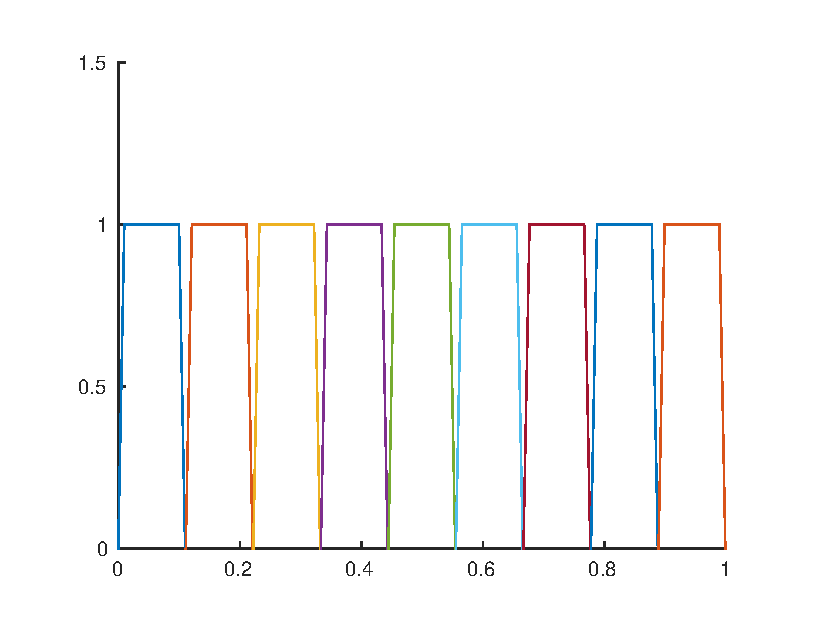
\includegraphics[width=.3\linewidth]{basis_constant.eps}}
  \label{fig:bspline_basis_constant}
\end{subfigure}%
\begin{subfigure}[B-spline basis for $p=1$]{
  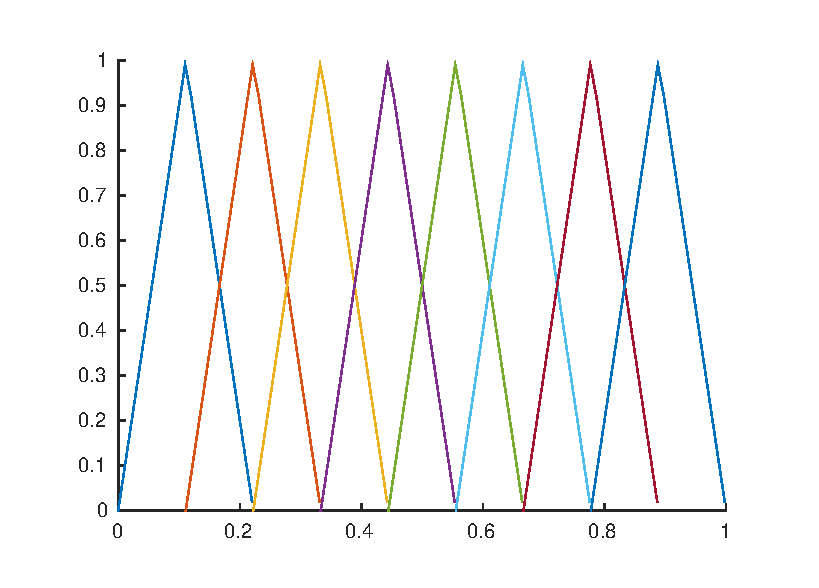
\includegraphics[width=.3\linewidth]{basis_linear.eps}}
  \label{fig:bspline_basis_linear}
\end{subfigure}
\begin{subfigure}[B-spline basis for $p=2$]{
  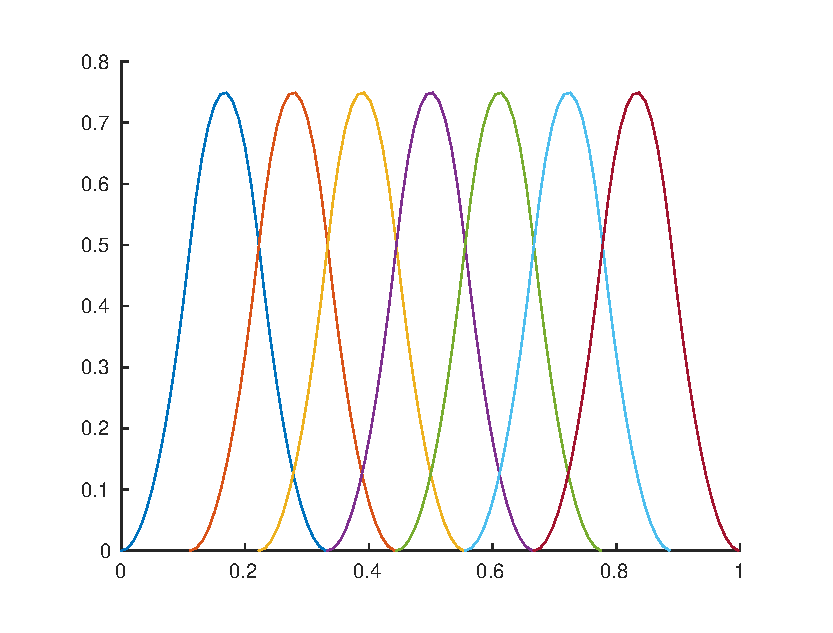
\includegraphics[width=.3\linewidth]{basis_quadratic.eps}}
  \label{fig:lognorm_quadratic}
\end{subfigure}
\caption{B-spline basis functions, of degree $p=0$ (left), $p=1$ (middle) and $p=2$ (right).}
\label{fig:bsplineBases}
\end{figure}


By giving each of these basis functions a weight $\omega_i$ and normalizing them at each point by dividing by the total sum, we get the rational basis functions. Writing them out explicitly, in terms of B-spline basis functions $N_{i,p}$, the $n^{\text{th}}$-degree NURBS curve with $k$ control points $P_i$ is finally given by:
\begin{equation}
C(u) = \frac{\sum_{i=1}^{k}N_{i,n}\omega_{i}P_{i}}{\sum_{i=1}^{k}N_{i,n}\omega_{i}}.
\end{equation}

B-splines are have the following properties, which are useful for our problem:
\begin{itemize}
\item Degree $n$ and number of control points $\vec{P}_{i\cdots m}$ are independent.
\item B-Splines only change locally (depending on the degree $n$) when a control point is changed.
\end{itemize}

Analogically to the Bezier curve surfaces, one can define B-spline or NURBS surfaces. For more information about NURBS see \cite{farin1999nurbs}.
%\subsection{Peters' Scheme for $G^1$ B{\'e}zier Surface Reconstruction}
\label{subsec:peters}
Although the process of generating a NURBS surface may seem trivial (placing the control points near the desired surface location), getting it to assume a specified shape can be quite a task. Generating a topology more complex than a torus \todointern{possible reference to figure above} requires several NURBS surfaces joined together. Thus, one needs to fulfil certain requirements in order for these surfaces to remain connected. For simple surface continuity ($C^0$), it is enough that the control points and knots on the edges of the two patches are the same, since then on both edges the surface follows a 1D--NURBS-curve from these points and knots. Smooth surfaces require higher-order continuity, which creates much more complex requirements. Several schemes have been created to automate such tasks.

The approach sometimes referred to as \emph{surface splines} or \emph{G-splines} \cite{eck1996automatic} solves the task of generating a smooth surface by starting from a \emph{control mesh} $\petersControlMesh$ of points, and computes B{\'e}zier surfaces by setting their control points to be linear combinations of the points in $\petersControlMesh$. The coefficients are determined such that the resulting surfaces will be \emph{tangent plane continous}, or $G^1$, or other desired degrees of smoothness.

One such scheme is the scheme of Peters, described in \cite{peters1992constructing}, which starts from an unstructured mesh of polygonal faces, and creates a $G^1$--continous surface from the location and connectivity of its vertices. This means that the normal vector to the plane is countinous, resulting in a smooth surface without sharp corners. The process consists of two steps, described below for a mesh of quadrilateral faces (quads) \cite{eck1996automatic}. However, the scheme could also be applied for a mesh with any mixture of polygons.

\subsubsection{Step 1: Mesh Refinement}
In the first step, the mesh is refined through two iterations of \emph{Doo-Sabin refinement}, as first described in \cite{DooSabin1978subdiv}. This refinement is done by creating new points $\vec{m}_{ref}$ around the vertices $\petersControlMeshVec$ in the control mesh $\petersControlMesh$. One such point is created for every face $f_{\vec{m}}$ that $\petersControlMeshVec$ corners, the new point $\vec{m}_{ref}$ being placed between $\petersControlMeshVec$ and the centroid $\centroidof{f_{\petersControlMeshVec}}$ of the bordering face $f_{\petersControlMeshVec}$ (the centroid of a face being the position of the face's vertices). After having done this for all the points in the control mesh $\petersControlMesh$, we group all the points $\vec{m}_{ref}$ into a new refined mesh $\petersControlMeshRef$. Describing this mathematically for the faces $\petersFaces$, with face ${\hat{f}}\in \petersFaces$ having vertices $V_{\hat{f}}$:

\begin{align}
\petersControlMeshRef =& \left\lbrace \petersControlMeshVec_{ref} \suchthat\petersControlMeshVec_{ref} = \alpha\petersControlMeshVec + (1-\alpha)\centroidof{f} \suchthat f \in \facesof{\petersControlMeshVec} \suchthat \right.
\\ \notag &
 \left. \suchthat \petersControlMeshVec \in \petersControlMesh, \alpha \in (0,1) \right\rbrace
\\
\where \qquad\qquad \centroidof{\hat{f}} =& \; \text{average}\left(\petersControlMeshVec_{\hat{f}}\right)_{\petersControlMeshVec_{\hat{f}} \in \verticesof{\hat{f}}}
\\
\text{and} \qquad\qquad F_{\vec{\hat{m}}} =& \left\lbrace \hat{f} \in \petersFaces \suchthat \vec{\hat{m}} \in \verticesof{\hat{f}}	\right\rbrace
\end{align}
where $\alpha$ is a smoothening parameter, controlling the sharpness of the corners and edges, which we for simplicity set to $1/2$, to get a simple midpoint.

Thus, in every refinement step on an $n$--gon, $n$ vertices are created, giving 4 vertices for a quad in the original control mesh. These are then joined up with the neighbours on the quad to form a smaller quad, and with the neighbouring points from the same vertex on the neighbouring quads, forming a quad along each edge. Around a quad corner, where $n$ quads meet (or $n$ edges in the general case), we instead get an $n$--gon around the corner vertex. After two refinements, we thus get a mesh of vertices $\petersControlMeshDobRef := \petersPatchPoints$ that mainly consists of quads, with possibilities of getting polygons with other number of edges around the vertices of the original mesh $\petersControlMesh$. The mesh and the resulting structure after two subdivisions can be seen in \autoref{fig:petersSubDivide}b.

\begin{figure}
	\centering
	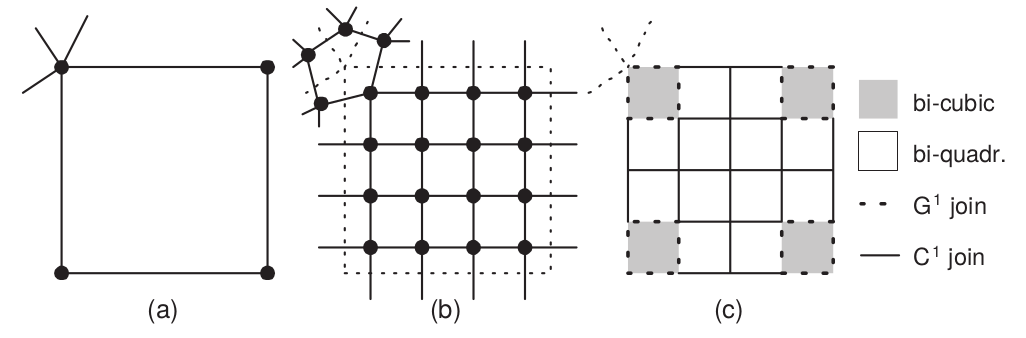
\includegraphics[width = \textwidth]{Pictures/NURBS/petersQuad_to_patches.png}
	\caption{The subdivision step in Peter's scheme. a): A quad in the original mesh, with edges and vertices marked out. Note that there are 5 edges connecting the top-left corner, making this a non-regular mesh corner. b): The mesh resulting from two Doo-Sabin subdivisions, denoted $\petersPatchPoints$ in the text. The mesh is regular, except for around the original mesh corners with other than 4 edges. In the case of the top-left corner, the 5 edges result in a pentagon. c): The resulting \Bez patch structure. The surface is at least $G^1$ continous everywhere. Figure from \cite{eck1996automatic}.}
	\label{fig:petersSubDivide}
\end{figure}

\subsubsection{Step 2: \Bez Patch Creation}
In this step, we create one \Bez patch for every vertex in the double refined mesh $\petersPatchPoints$. 

To begin with, we can recognize that each original quad now has a $4 \times 4$ grid of vertices, where the $4$ vertices along each original quad edge match the $4$ vertices on the neighbouring quad (see \autoref{fig:petersSubDivide}b). From this, we see that most of the cells will be locally in a regular grid, in the sense that it can be seen as the center grid point in a $3\times3$ \todointernal[author=Benni]{which $3\times3$ grid? I thought its $4\times4$...Is it the red grid in Fig. 2.4.3 a)?}two-dimensional structured grid. For illustration, we can look at \autoref{subfig:peterspoints}, where this $4 \times 4$ grid of vertices is marked with black or green crosses. Here, the green crosses illustrate one such local neighbourhood, where the green point in the middle of the darker patch $\petersLocalPatchPointIndices{0,0}$ can be seen as the centre point of the $3 \times 3$ green points $\petersLocalPatchPointIndices{i,j}$, $i,j \in \left \lbrace-1,0,1\right \rbrace$, around it (although the global mesh might look very different further away).% have $8$ local neighbours ($4$ along the edges of the double refined quads, and $4$ along the diagonals of the doubly refined quads). 

Now, for any of these local neighbourhoods of $3\times3$ points $\petersLocalPatchPointIndices{i,j}$, $i,j \in \left \lbrace-1,0,1\right \rbrace$, we can now interpret them as the control points for a biquadratic (that is, second-order) tensor product B-spline surface (meaning with uniform knots). If a neighbouring point is also in a locally regular  $3\times3$ point neighbourhood, we could then extend the B-spline surface to this local neighbourhood by adding them as control points in that direction, using some extra knots. This way, we could build up a network of patches using all the points that are also locally in a regular grid (and their neighbours in their own local $3\times3$ grid). This would results in a $C^1$ continous surface around all vertices where the mesh is locally regular.
%For those cells, we can now create biquadratic tensor splines that meet $G^1$ along the edges and corners; that is, the tensor product of one quadratic spline in one of the regular mesh directions and one in the other.
Now, this surface can also be represented by a network of a biquadratic tensor product \Bez surface patches (see \autoref{fig:petersSubDivide}c for the patch structure), which we will use to describe the whole surface. This means, around a vertex $\petersLocalPatchPointIndices{0,0}$, we create \Bez surface, with $3\times3$ control points for each patch, that we choose to call $\petersLocalBezPointIndices{i,j}$ ($i,j \in \left \lbrace{-1},0,1\right \rbrace$). If we do this, the $3\times3$ \Bez control points $\petersLocalBezPointIndices{i,j}$ will lie at positions in-between the center vertex $\petersLocalPatchPointIndices{0,0}$ and the $3\times3$ local grid vertices $\petersLocalPatchPointIndices{i,j}$, as shown in \cite{peters1992constructing}:
\begin{equation}
\petersLocalBezPointIndices{i,j} = \frac{1}{4}\left(\petersLocalPatchPointIndices{i,j} + \petersLocalPatchPointIndices{i,0} + \petersLocalPatchPointIndices{0,j} + \petersLocalPatchPointIndices{0,0}\right)
\end{equation}
or, writing it out explicitly for $i,j \in \left \lbrace{-1},0,1\right \rbrace$,

\begin{scriptsize}
\begin{align*}
\petersLocalBezPointIndices{{-1},1\phantom{-}} =&\, \frac{1}{4}\left(\petersLocalPatchPointIndices{{-1},1} + \petersLocalPatchPointIndices{{-1},0} + \petersLocalPatchPointIndices{0,1} + \petersLocalPatchPointIndices{0,0}\right)
&
\petersLocalBezPointIndices{0,1\phantom{-}} =&\, \frac{1}{2}\left(\petersLocalPatchPointIndices{0,1} + \petersLocalPatchPointIndices{0,0}\right)
&
\petersLocalBezPointIndices{1,1\phantom{-}} =&\, \frac{1}{4}\left(\petersLocalPatchPointIndices{1,1} + \petersLocalPatchPointIndices{1,0} + \petersLocalPatchPointIndices{0,1} + \petersLocalPatchPointIndices{0,0}\right)
\\
\petersLocalBezPointIndices{{-1},0\phantom{-}} =&\, \frac{1}{2}\left(\petersLocalPatchPointIndices{{-1},0} +  \petersLocalPatchPointIndices{0,0}\right) 
&
\petersLocalBezPointIndices{0,0\phantom{-}} =&\,\phantom{\frac{1}{2}\Bigl(} \petersLocalPatchPointIndices{0,0}\phantom{\Bigr)}
&
\petersLocalBezPointIndices{1,0\phantom{-}} =&\, \frac{1}{2}\left(\petersLocalPatchPointIndices{1,0} + \petersLocalPatchPointIndices{0,0}\right)
\\
\petersLocalBezPointIndices{{-1},{-1}} =&\, \frac{1}{4}\left(\petersLocalPatchPointIndices{{-1},{-1}} + \petersLocalPatchPointIndices{{-1},0} + \petersLocalPatchPointIndices{0,{-1}} + \petersLocalPatchPointIndices{0,0}\right) 
&
\petersLocalBezPointIndices{0,{-1}} =&\, \frac{1}{2}\left(\petersLocalPatchPointIndices{0,{-1}} + \petersLocalPatchPointIndices{0,0}\right)
&
\petersLocalBezPointIndices{1,{-1}} =&\, \frac{1}{4}\left(\petersLocalPatchPointIndices{1,{-1}} + \petersLocalPatchPointIndices{1,0} + \petersLocalPatchPointIndices{0,{-1}} + \petersLocalPatchPointIndices{0,0}\right)
\end{align*}
\end{scriptsize}

\begin{figure}
\begin{center}
\begin{subfigure}[b]{.49\textwidth}
\begin{center}
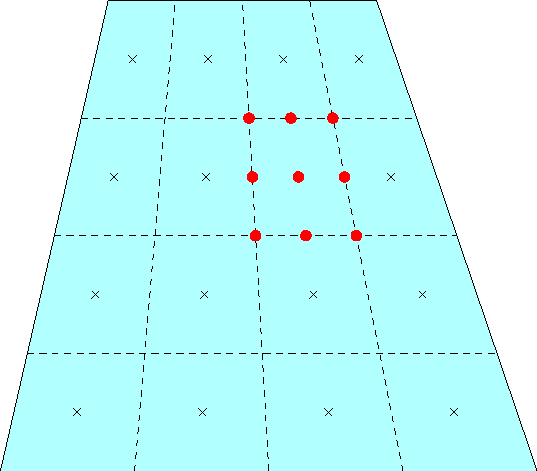
\includegraphics[width=.9\textwidth]{Pictures/NURBS/bezier_points.pdf}
\subcaption{Different points on a quad.}
\label{subfig:peterspoints}
\end{center}
\end{subfigure}
~
\begin{subfigure}[b]{.49\textwidth}
\begin{center}
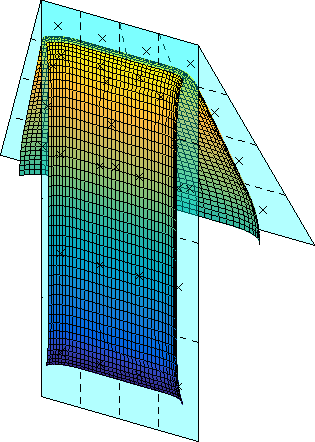
\includegraphics[height=\textwidth]{Pictures/NURBS/bspline_patches.pdf}
\subcaption{Smoothly connected \Bez patches.}
\label{subfig:smoothsurf}
\end{center}
\end{subfigure}
\caption{(\subref{subfig:peterspoints}): The different points used in Peter's scheme. For the quad in the picture with vertices $A,B,C,D$ in $\petersControlMesh$, the refined mesh vertices in $\petersPatchPoints$ created by two Doo-Sabin refinements are marked out with crosses. The extent of each of their \Bez surface patches is also marked on the quad with dotted lines (see \autoref{fig:petersSubDivide}b,c for comparison). Additionally, for the highlighted patch, the tensor product \Bez surface points $\petersLocalBezPointIndices{i,j}$ are marked with red circles, with the corresponding refined mesh points $\petersLocalPatchPointIndices{i,j}$ being the green crosses. (\subref{subfig:smoothsurf}): The resulting smoothly connected surface after creating \Bez surface patches. For visibility, two quads have been cut-out, although the surface is part of a bigger figure. The refined points in $\petersPatchPoints$ are again marked with crosses.}
\label{fig:petersDiags}
\end{center}
\end{figure}

The creation of these different types of points is also illustrated in \autoref{subfig:peterspoints}. 


%as following (see [\todointern[inline]{ref to figure with names on points, EckHoppe or Peters}] for nomenclature):
%%
%\begin{equation}
%
%\end{equation}
%%
To summarize, we have thus just created a surface around all the vertices that are locally in a regular mesh. The exceptions that cannot be placed as such, are now the points residing on the corners of the original quads, since any number of quads may be meeting there.
%This comes from the fact that at quad corners, we may have any number of quads meeting, starting from 3. 
For $n$ quads sharing a corner vertex, the refinement steps will create a polygon with $n$ sides, as mentioned above. If $n\neq4$, the vertices of these corner polygons cannot be placed in a locally regular mesh, and we cannot apply the previous technique -- see for example the upper-left corner of \autoref{fig:petersSubDivide}b.

However, we can still create a \Bez patch which connects smoothly to the locally regular points. To do this, we create a bicubic \Bez patch (of polynomial order 3, one higher than around the regular points, meaning it has $4\times4$ control points) for every vertex in the corner polygon.
We then evaluate how the surface position and normal direction depends on the \Bez control points along all edges of the patches. In order to have a smooth connection, we want these to match, and thus, we can produce constraints for the positions of the \Bez control points.
Since the surfaces are defined at each point as linear combinations of the \Bez control points (which in turn are linear combinations of the vertices in the doubly refined mesh $\petersPatchPoints$), the constraints result in an underdetermined system of linear equations for all the \Bez control points on the bicubic \Bez patches on the vertices in the doubly refined mesh $\petersPatchPoints$.

As the resulting formulae for the locations of the \Bez control points are rather lengthy and complex, we refer to the original paper (ref. \cite{peters1992constructing}). Here, it is also proven that the surfaces have an overall $G^1$ connectivity. A cut-out sample can be seen in \autoref{subfig:smoothsurf}.

To summarize, Peters' scheme is a mathematical algorithm for creating biquadratic and bicubic \Bez patches that join with $G^1$ continuity, from a mesh of polygons. Firstly, a set of refined mesh points is created on each polygon. Then, \Bez control points defining the patches are created as linear combinations of the vertices in this refined mesh. The $G^1$ continuity results from the interpretation of the refined mesh as a regular biquadratic tensor product B-spline surface, and where this is not possible, bicubic \Bez patches are constrained to join smoothly to the surrounding biquadratic patches.
%In this section we will cover the following, referring to \cite{peters1992constructing}:
%\begin{itemize}
%\item How we go from polygonal faces to a set of mesh control points. "patch points", specifying that we're talking about quads, and that we then get 16
%\item That for each of these 16 points, we will make a small B{\'e}zier patch
%\item That if we define the B{\'e}zier control points of these patches in a special way, as described in appendix XYZ \todointern{TODO: create this appendix, or change this to refer to paper for coefficients}, we get a surface that is $G^1$ continous
%\item Maybe describe that we then need for every one of these B{\'e}zier patches the locations of the neighbours
%\item That the location of a point on the surface defined by parameters $\vec{s} = (u,v)$ depends on the B{\'e}zier control points, whose linear dependence on the "patch points" give us coefficients on these "patch points" of the location described by the parameters, as can be seen in \autoref{fig:PetersPoints}
%
%\end{itemize}


%\begin{figure}
%
%\missingfigure{Graphical description of all those different points in Peters' Scheme}
%\label{fig:PetersPoints}
%\caption{The points in Peters' Scheme. As clearly seen in the figure above, this scheme is self-explanatory.}
%\end{figure}
